%!TEX encoding = UTF-8 Unicode
%!TEX root = ../thesisCASes.tex

%% TITOLO
\section{Introduzione}
\label{sec:Introduzione}

Nel corso del XX secolo, il mondo scientifico ha subito importanti cambi di paradigma. 
In particolare, durante la Seconda Guerra Mondiale, 
si è assistito all'emergere di una nuova prospettiva scientifica consolidata al termine del conflitto,
la nascita della cibernetica e la conseguente formulazione
di scienze della complessità.
La complessità, non è un ambito trattato da una sola scienza,
ma più un nuovo modo di pensare e di osservare i fenomeni
della realtà. \\
Se nella cosmologia greca la realtà veniva spiegata come caos per 
l'insieme disordinato e indeterminato degli elementi materiali, 
contrapposto al cosmos che rappresentava l'ordine, 
come si può osservare fra i miti delle varie Teogonie
fra cui la più famosa quella scritta da Esiodo, \footcite{esiodoteogonia}
oggi la complessità ci spinge a riconsiderare questa dicotomia e a sviluppare 
nuovi strumenti per comprendere la realtà. 
Il caos, anzi il caos deterministico, è infatti la scienza che studia i 
sistemi dinamici che esibiscono una sensibilità esponenziale rispetto alle condizioni iniziali.
O, in termini più rigorosi, è la scienza che studia la dinamica dei sistemi non lineari.
Questo cambio di paradigma ha avuto inizio verso la fine del XIX secolo,
quando uno studioso nell'ambito della meccanica classica, Henri Poincaré,
osservò e analizzò la possibilità di un comportamento fortemente irregolare
di alcuni sistemi dinamici studiando il problema dei tre corpi,
che lo portò alla scoperta del caos matematico. \footcite{poincaréproblema}
La scoperta di Poincaré segnerà un punto di svolta che verrà
ripreso poi solamente a metà del secolo successivo dal meteorologo
Edward Norton Lorenz,
quando nel '63 Lorenz pubblicherà il suo articolo 
\textit{Deterministic Nonperiodic Flow} \footcite{Lorenzdnf},
nel quale tratta del comportamento caotico in un sistema semplice
e deterministico, con la formazione di un attrattore strano,
e aprendo di fatto ufficialmente la strada quella che diverrà poi
la famosa teoria del caos.
Mostrando come in realtà all'interno dell'ordine emergano forme di disordine,
e all'interno del disordine siano presenti forme di ordine. \\
Prima dell'introduzione di questa tesi, si rende comunque necessario
qualche chiarimento e qualche informazione 
preliminare per comprendere cosa s'intenda con certi termini che ritroveremo
nel corso della tesi, e questi sono la nozione di sistema dinamico e di sistema complesso.
Un sistema dinamico è un modello matematico che rappresenta un oggetto (sistema),
con un numero finito di gradi di libertà che evolve nel tempo secondo una legge
deterministica; Mentre per sistema complesso si intende un sistema dinamico a multicomponenti,
ovvero composto da diversi sottosistemi che solitamente interagiscono fra loro.
Tipicamente un sistema dinamico viene rappresentato analiticamente da un’equazione
differenziale, espressa poi in vari formalismi, e identificato da un vettore nello
spazio delle fasi: lo spazio degli stati del sistema, dove "stato" `e un termine che
indica l’insieme delle grandezze fisiche, dette variabili di stato, i cui valori
effettivi "descrivono" il sistema in un certo istante temporale.

\subsection{La Cibernetica}
\label{sec:La Cibernetica}
Rintracciando l'origine di questi termini è necessario tornare 
a questo complesso scenario del XX secolo,
più precisamente al termine della seconda guerra mondiale e
qualche decennio prima della formulazione della teoria del caos,
in quel periodo uno dei più importanti avanzamenti nelle scienze che contribuì alla
formazione del primo paradigma della complessità,
risiedette nell'introduzione della cibernetica. \\
La cibernetica è la scienza che studia i principi astratti di organizzazione
nei sistemi complessi, ed ebbe inizio durante gli anni della seconda guerra
mondiale, merito del fisico e matematico Norbert Wiener.
Nel '40 Wiener insieme ad altre ad altre prominenti figure provenienti
da diversi ambiti scientifici,
come Ross Ashby, Margaret Mead, Gregory Bateson, Heinz von Foerster,
partecipano ad una serie di conferenze
multidisciplinari chiamate "The Macy Conferences", inizialmente intitolate come
"Feedback Mechanism in Biology and the Social Sciences"
con l'obiettivo comune di andare a definire
gli ambiti di interesse della nuova scienza.
A seguito nel '48,
ispirato dalla meccanica ed i suoi risultati conseguiti durante la guerra
e contemporaneamente dallo sviluppo della teoria della comunicazione
(o informazione) di Claude Shannon,
con la volontà di sviluppare una teoria generalizzata dei principi di
organizzazione e controllo nei sistemi emersi durante le conferenze,
pubblicherà un libro:
La cibernetica, controllo e comunicazione nell'animale e nella macchina;
in cui definiva l'ambito di interesse e gli obiettivi della nuova disciplina
inaugurando anche l'uso del nuovo termine da lui coniato.
A seguito di questo libro che riscuoterà
un importante successo, le conferenze presero il nome di
"Cybernetics, Circular Causal, and Feedback Mechanism
in Biological and Social Systems", \footcite{fabbrisgiustinianocyb}
riconoscendo Wiener come la principale figura di spicco della nuova scienza. \\
In particolare come evidenziato fino ad ora dalla sua natura multidisciplinare,
la cibernetica non si interessa di individuare in
cosa consistano questi sistemi,
ma più che altro di comprenderne il loro funzionamento. \\
Le fortunate premesse iniziali della cibernetica risiedevano in una convinzione
da parte di questi scienziati provenienti dai differenti ambiti disciplinari,
che esistesse uno "schema processuale" comune ad organismi viventi e macchine,
rintracciato attraverso una ricerca uniforme
garantita dall'utilizzo di un metodo
“sintetico” e

\todo[inline,color=green]{le virgolette si aprono e si chiudono con simboli diversi. ti ho corretto sintetico ma cerca di correggerle tutte. alt+2 per aprirle e shift+alt+2 per chiuderle.}

"comportamentale". 
L'aspetto meta-disciplinare del pensiero cibernetico,
esplicito nella sua fondazione, godrà però di una fama più popolare 
che conseguirà in importanti realizzazioni 
tra l'inizio degli anni '60 e la metà del '70, 
grazie al contributo degli scienziati:
Heinz von Foerster, Margaret Mead, Gregory Bateson, e altri;
proprio in quel periodo si compieranno ulteriori passi fondamentali che porteranno
il pensiero sistemico verso un consolidamento di una scienza più concreta.
Uno dei casi più rilevanti di quel periodo, è il passaggio da una "cibernetica di primo ordine"

\todo[inline,color=green]{in generale non puoi usare le virgolette con molteplici scopi. se le usi per i modi di dire non puoi usarle per le citazioni e nemmeno per le frasi chiave o importanti.}

a una "cibernetica di secondo ordine", anche chiamata come "la cibernetica dei sistemi di osservazione",
questa distinzione si deve a Heinz Von Foerster, 
che è stato uno scienziato e filosofo austriaco noto per i suoi contributi 
alla cibernetica e alla teoria della comunicazione. \footcite{scottsecondordercyb}
Vi sono alcune differenze sostanziali nel passaggio da cibernetica di primo ordine a quella di secondo ordine, 
nel primo periodo lo studioso di cibernetica (di primo ordine)
studiava un sistema da un punto di vista passivo, da quello dell'osservatore
dei comportamenti del sistema, senza tener conto della propria influenza 
nei casi di studio.
Il cibernetico di secondo ordine invece, è consapevole della propria 
influenza all'interno del sistema, riconoscendo il sistema come un agente con cui interagire, 
e riconoscendo esso stesso come agente nell'interazione col sistema, 
e di conseguenza proprio come spiega Heinz Von Foerster nei suoi scritti,
di come la realtà per come la percepiamo possa esistere
soltanto se si tiene conto del fatto che la sua rappresentazione è fortemente dipendente 
dall'esistenza di un ambiente che racchiude il sistema stesso. \footcite{understandingunderstanding}
In altre parole, l'ambiente non esiste in sé, ma viene creato dalla relazione 
tra l'osservatore e ciò che viene osservato.
Questa teoria ha importanti implicazioni per la cibernetica, 
poiché sottolinea l'importanza dell'interazione tra il sistema e il suo ambiente 
nella comprensione del funzionamento del sistema stesso. 
Inoltre, sottolinea l'importanza di considerare la prospettiva 
dell'osservatore nell'analisi dei sistemi e dei processi.
In conclusione, nella visione di Foerster, 
l'organizzazione ed eventuale disorganizzazione di alcun sistema può esistere 
se questo non viene studiato prendendo in considerazione l'ambiente che lo racchiude.
A partire dunque da queste importanti premesse, e dalle conseguenze 
che la cibernetica ha avuto in tutti gli ambiti delle scienze, è doveroso 
notare che questa ha avuto un ruolo centrale nello sviluppo di
molti studi scientifici e la nascita
di nuovi ambiti come: l'intelligenza artificiale, la teoria del caos,
la teoria della catastrofe,
la teoria dei controlli, la teoria generale dei sistemi, la robotica,
la psicologia, le scienze sociali, e molto altro 
(perfettamente in accordo con la sua natura multidisciplinare).

\subsection{Le Cibernetiche nella musica}
\label{sec:Le cibernetiche nella musica}
All'inizio degli anni '60, in seno alle nascita delle scienze complesse,
l'uso di sistemi di \emph{feedback} \todo[inline,color=green]{sarebbe opportuno mettere in un campo \emph{} le parole che lasci in inglese e che non sono in uso nella lingua italiana} e la rilevanza dei circuiti informativi chiusi
nelle strutture organizzate
ha goduto di uno slancio popolare anche nel mondo della musica
e più in generale dell'arte. \\
Tuttavia come vedremo, a parte casi popolari di deliberate dichiarazioni
formali da parte degli artisti, non bisogna pensare ai lavori che andremo a citare
come atti pionieristici che sanciscono una volta per tutte la nascita della cibernetica in musica,
ma è più corretto pensare alle questioni sistemiche come ad una sensibilità
comune condivisa in un certo periodo da diversi autori provenienti da diverse parti del mondo,
che sono stati influenzati e si sono influenzati a vicenda
con le stesse idee per un interesse condiviso riguardo
le teorie cibernetiche di Weiner e delle Macy Conferences. \\
% Europa - Roma
In Europa nel '51, Herbert Eimert, Werner Meyer-Eppler e Robert Beyer
di comune accordo con il direttore della NWDR, Hanns Hartmann,
attrezzarono e crearono quello che divenne il primo studio per la Musica Elettronica. 
\footcite{discipiocircuitideltempo}
Questo divenne lo studio più influente al mondo durante gli anni '50 e '60,
con ospiti alcuni dei più importanti compositori contemporanei provenienti da tutta Europa,
come Franco Evangelisti, Karlheinz Stockhausen, György Ligeti, Roland Kayn, Herbert Brün,
Cornelius Cardew, e molti altri.
In quel periodo il lavoro di ricerca condotto da Werner-Meyer Eppler,
scienziato, musicista, fra gli ideatori e direttori dello studio di Colonia e
direttore dell'istituto di fonetica all'università di Bonn,
pone una certa attenzione in quelle che furono le prime
teorizzazioni della teoria dell'informazione e della cibernetica,
che porteranno l'autore alla scrittura di importanti testi di ricerca.
Fra le altre cose Werner-Meyer Eppler nel '50 escogita un uso particolare
del magnetofono, mediante retroazione \textit{(feedback)} fra le testine di riproduzione e 
registrazione, creando a tutti gli effetti una prima forma di \textit{tape delay}. \footcite{discipiocircuitideltempo}
Dalle esperienze dello studio di Colonia ne usciranno molti compositori interessati
alle teorie cibernetiche. \\
Un caso importante in questo scenario è quello del compositore Roland Kayn,
Il progetto di musica cibernetica di Kayn ha ricevuto il suo impulso iniziale
quando nel '53, ad allora giovane musicista e studente universitario,
venne in contatto con il filosofo Max Bense professore all'Università Tecnica di Stoccarda.
Subito dopo il suo primo incontro con Bense sempre nel '53, Kayn entrò in contatto con Herbert
Eimert presso lo studio elettronico della Westdeutscher Rundfunk di Colonia.
Roland Kayn era affascinato dal potenziale sonoro offerto dalle nuove tecnologie,
ma trovava che l'estetica serialista dominante nello studio in quegli anni
era per lui qualcosa di troppo restrittivo, esperienza che lo portò
per i successivi dieci anni a concentrarsi
principalmente sulla composizione strumentale e le applicazioni delle teorie
cibernetiche in modo formale. \footcite{thomaswpattesonkayn}
Sempre in quel periodo, sostanzialmente diverso e altrettanto importante
è il caso di Franco Evangelisti, che dopo essersi avvicinato alla musica elettronica
anche lui sotto la guida e su invito di Herbert Eimert, allo studio elettronico
della Westdeutscher Rundfunk di Colonia nel '56,
iniziò le sue ricerche che dopo un anno e mezzo di intenso lavoro lo portarono
al completamento della sua forse più importante composizione elettronica:
Incontri di fasce sonore, trasmessa da Radio Colonia nel '57.
Nel '59, Evangelisti è nuovamente in Italia, dove fu tra i promotori
della settimana internazionale di nuova musica a Palermo.
L'anno seguente, assieme ad altri musicisti
fondò l'associazione Nuova Consonanza, con lo scopo di diffondere
la musica contemporanea italiana e straniera con concerti convegni ed eventi di vario tipo.
Dall'associazione nacque più tardi l'omonimo Gruppo di improvvisazione 
(GINC: Gruppo d'Improvvisazione Nuova Consonanza)
che allora veniva presentato come "il primo ed unico gruppo formato da compositori-esecutori"
e che permise ad Evangelisti di mettere in pratica le proprie teorie sull'improvvisazione,
riguardo queste citerà più volte deliberatamente in interviste, scritti,
e altre documentazioni, il suo approccio sistemico/cibernetico
in quelle che saranno le esperienze con il Gruppo.\footcite{GINCAzioni} \\
Nel '60 si trasferisce a Roma Roland Kayn da vincitore del Prix de Rome,
dove dal '64 assieme ad Aldo Clementi e Franco Evangelisti
prende parte al Gruppo di improvvisazione Nuova Consonanza
del quale fece parte sino al '68,
ed è in quel periodo che Kayn ispirato dalle teorie della cibernetica iniziò a sperimentare
estensivamente con sistemi di autoregolazione basati su feedback loop,
non più solo come modelli formali per composizioni strumentali
ma anche come reti di generatori di segnale analogici. \\
% Europa - Francia
In questo scenario, sempre negli anni '50 in Europa, uno dei primi artisti nella storia dell'arte
ad evocare l'uso della cibernetica nei propri lavori è stato
Nicolas Schoeffer con il suo ciclo di lavori "spazio-dinamici", in acronimo
CYSP - Cybernetic Spatiodynamic.
In particolare Schoeffer ha creato la prima installazione ad implementare meccanismi
di auto-regolazione, il CYSP-1 \footcite{sanfilippovallefeedsys},
capace di essere sensibile all'ambiente esterno e a se stesso
grazie ad una serie di tecnologie offerte dalla compagnia Philips (fotocellule e microfoni),
questa prima scultura spazio-dinamica, è dotata di totale autonomia di movimento
(viaggio in tutte le direzioni a due velocità) e di rotazione assiale ed eccentrica
(messa in moto delle sue 16 lastre policrome pivotanti),
ed era capace di reagire sonoramente a questi stimoli riproducendo
una serie di registrazioni composte dal compositore francese Pierre Henry,
collaboratore di Pierre Schaeffer ed insieme a lui figura centrale nella nascita della musique concrète.
Questa scultura viene celebrata come una prima opera di carattere cibernetico 
entrata a far parte nel mondo dell'arte.

% America
Cambiando continente e passando dall'Europa ad osservare cosa stava accadendo
in America in quegli anni, troveremo tanti altri rilevanti atti pioneristici,
come ad esempio quelli che sono stati i lavori di Louis e Bebe Barron.
I due (marito e moglie) furono compositori e pianisti che si
interessarono alla musica elettronica sin dal periodo della sua origine.
Intorno al '50 i due si trasferirono al Greewitch Village a New York
dove furono attivi in collettivi di musica sperimentale
collaborando con persone come John Cage ed altri.
I Barron trasformarono
la loro casa in una specie di studio di musica elettronica
dove scrivevano soundtracks per film sperimentali.
Per Louis e Bebe il grande passo arrivò nel
'56, quando i due si ritrovarono a scrivere la soundtrack per il film:
\textit{Forbidden Planet},
questo sarà il primo film mainstream di Hollywood ad utilizzare una soundtrack
composta solamente ed interamente da elettronica.
L'elettronica di \textit{Forbidden Planet} è stata
costituita a partire da dei circuiti appositamente creati da i due compositori,
che deliberatamente ispirati dalle teorie cibernetiche di Wiener
dichiareranno: \footcite{dunbarlisteningcyb}

\todo[inline,color=green]{LUCA! le citazioni sono le perle di un testo di tesi. tu scegli le parole degli altri che vuoi mettere tra le tue! cristo santo centrate in corsivo come se fosse un biglietto degli auguri di natale! LUCA!!!! ! ! !}

%\begin{center}
%\vspace{0.5cm}
%\textit{What we did was pretty elementary: we would attach resistors and capacitors
%to activate these
%circuits... negative and positive feedback was involved - Wiener
%talks about all that. The same
%conditions that would produce breakdowns and malfunctions in machines,
%made for some
%wonderful music. The circuits would have a “nervous breakdown”
%and afterwards they would be
%very relaxed, and it all came through in the sounds they generated.}
%\vspace{0.5cm}
%\end{center}

\begin{quote}
What we did was pretty elementary: we would attach resistors and capacitors
to activate these
circuits... negative and positive feedback was involved - Wiener
talks about all that. The same
conditions that would produce breakdowns and malfunctions in machines,
made for some
wonderful music. The circuits would have a “nervous breakdown”
and afterwards they would be
very relaxed, and it all came through in the sounds they generated.
\end{quote}

I circuiti in retroazione erano destinati al corto circuito,
e utilizzati appositamente come materiale per la generazione acustica
di trame incise su nastro.
Altri importanti compositori di quel periodo sono al lavoro su composizioni
che sfruttano sistemi di feedback, fra i più rilevanti:
John Cage, David Tudor, Robert Ashley, Gordon Mumma e Steve Reich. \footcite{sanfilippovallefeedsys} \\
Fra questi David Tudor è stato uno dei primi musicisti a montare uno dei primi esempi di un sistema strumentale
basato su feedback complessi, per la realizzazione di Variations II (1960) di John Cage,
mentre Gordon Mumma nel 1966 si aggrega alla compagnia di Merce Cunningham per il quale compone Mesa, 
una prima improvvisazione "Cybersonic" per David Tudor; da lì in poi comporrà importanti 
brani e improvvisazioni cibernetiche negli anni a venire, come ad esempio Hornpipe (1967), 
che nasce dall'interazione fra performer, uno strumento cibernetico e la risonanza della sala di esecuzione: 
al corno francese e' collegata una console che si sintonizza sul feedback 
della sala e reagisce ai suoni emessi dallo strumento. \\
Un secondo periodo costituito da un approccio sistemico più consapevole
che inizia a tracciare la strada per un pensiero ecosistemico della composizione,
in un certo senso si può affermare che inizi dal lavoro
di Alvin Lucier, che nel '69 scriverà quello che sarà un brano emblematico per
le cibernetiche in musica \textit{I'm sitting in a room},
che è un brano importante per quelle che sono
le logiche di interazione sistemiche fra uomo/macchina/ambiente che approfondiremo 
più avanti nel corso della tesi,
e che proprio come nel passaggio da cibernetica di primo 
ordine a quella di secondo ordine di cui parla Heinz Von Foerster, 
viene sancita l'interazione sistemica dove il musicista l'ambiente e lo strumento
divengono parti di un insieme complesso;
il sistema stesso di \textit{I'm sitting in a room} si osserva tramite l'ambiente 
nel corso della sua evoluzione, tracciando una storia di relazioni e interazioni 
con questo.
Nel brano di Lucier, un performer
recita in un microfono un testo che descrive il fenomeno che avverrà poco a poco,
la voce recitante nel microfono viene registrata e poi riprodotta da altoparlanti
posti nella stanza, il suono della registrazione riprodotta da questi altoparlanti
viene poi registrato nuovamente durante la riproduzione da un secondo supporto, e l'operazione
viene ripetuta con questa casualità circolare di volta in volta
fino alla fine, dove rimarranno
solamente: i contributi provenienti dalle frequenze di risonanza della stanza,
dalla voce, e dalla catena elettroacustica,
dando vita nel loro insieme ad un processo molto lento di feedback positivo dove
la natura stessa non lineare del processo e degli agenti porterà di volta in volta ad un risutato
sempre differente.
Lucier racconta di essere stato originariamente ispirato
a creare I Am Sitting in a Room dopo aver partecipato a una conferenza al MIT,
in cui Amar Bose, imprenditore, ingegnere elettrico e tecnico del suono,
descrisse come testava le caratteristiche degli altoparlanti
che stava sviluppando, ri-diffondendo l'audio prodotto nella stanza e poi
riprendendolo tramite i microfoni, in quella che è la stessa casualità
circolare ripresa ed utilizzata artisticamente da Lucier. \footcite{lucierbose} 
Dopo l'esperienza di Lucier, Nicolas Collins,
formatosi nella tradizione compositiva sperimentale con: Alvin Lucier,
David Behrman e David Tudor, con i quali ha lavorato a stretto contatto,
nel '74 compone il brano \textit{Pea Soup} mentre è studente alla Wesleyan University.
In \textit{Pea Soup} una rete auto-stabilizzante di circuiti analogici
(originariamente tre Countryman Phase Shifter)
sposta il tono del feedback elettoacustico su una frequenza di risonanza
diversa ogni volta che questo si inizia a
costruire. Il suono familiare del fenomeno è sostituito da schemi instabili
che danno vita ad un raga site-specific
rispecchiando la personalità acustica della stanza. \footcite{collinspeasouphist}
Anche in questo lavoro appare chiaro come una certa sensibilità
nei confronti del fenomeno di feedback si stia avvicinando ad una logica più vicina
a quella della cibernetica di secondo ordine.
Per citare un'ultima esperienza americana rilevante,
c'è infine il caso della neural synthesis di David Tudor.
David Tudor nel '89 incontrò il progettista e designer Forrest Warthman
dopo uno show a Berkeley,
che che lo introdusse all'idea di utilizzare reti neurali analogiche
per combinare tutta la sua complessa attività live-electronics in un unico computer.
\footcite{tudorneuralsynth}
Uno dei risultati è apprezzabile nei CD's "Neural Synthesis", 
in uno di questi sono presenti delle importanti note di copertina di Warthman:

\begin{quote}
This recording combines the art of music, the engineering of electronics,
and the inspiration of biology. In it,
David Tudor orchestrates electronic sound in ways analogous to
our biological bodies' orchestration of consciousness...
The neural-network chip forms the heart of the synthesizer.
It consists of 64 non-linear amplifiers (the electronic neurons on the chip)
with 10240 programmable connections.
Any input signal can be connected to any neuron,
the output of which can be fed back to any input via on-chip or off-chip paths,
each with variable connection strength. The same floating-gate devices used in EEPROMs
(electrically erasable, programmable, read-only memories)
are used in an analog mode of operation to store the strengths of the connections.
The synthesizer adds R-C (resistance-capacitance) tank circuits on feedback
paths for 16 of the 64 neurons to control the frequencies of oscillation.
The R-C circuits produce relaxation oscillations.
Interconnecting many relaxation oscillators rapidly produces complex sounds.
Global gain and bias signals on the chip control the relative amplitudes of neuron oscillations.
Near the onset of oscillation the neurons are sensitive to inherent
thermal noise produced by random motions of electron groups moving through
the monolithic silicon lattice. This thermal noise adds unpredictability
to the synthesizer’s outputs, something David found especially appealing.
The synthesizer’s performance console controls the neural-network chip.
R-C circuits, external feedback paths and output channels.
The chip itself is not used to its full potential in this first synthesizer.
It generates sound and routes signals but the role of learner,
pattern-recognizer and responder is played by David, himself a vastly
more complex neural network than the chip \\
(Neural Synthesis No.6-9 liner notes by Forrest Warthman, Palo Alto 1995
\footcite{http://www.lovely.com/albumnotes/notes1602.html})
\end{quote}

Oggi molti compositori, italiani e non, 
applicano un approccio sistemico alla composizione musicale elettroacustica, 
ispirandosi alle trame delineate dalle scienze delle complessità e dai lavori citati. \\
Tra i compositori che si sono distinti in questo campo, 
uno dei maggiori è Agostino Di Scipio, 
che fin dagli anni '90 ha dedicato i suoi studi al caos e ai sistemi complessi, 
prima in modo formale \footcite{discipioiterated}, per iniziare poi successivamente, 
verso la metà degli anni '90, il lavoro sulla composizione ecosistemica con il suo ciclo di lavori 
- ecosistemico udibile, che come vedremo a seguito riprende le tematiche della cibernetica di secondo ordine, 
dove il sistema si osserva tramite l'ambiente circostante.
Altri compositori di rilievo includono Dario Sanfilippo, 
compositore e ricercatore che ha studiato con Agostino Di Scipio e con all'attivo 
importanti pubblicazioni e lavori nell'ambito dei sistemi autonomi DSP in musica. 
Le sue tematiche rimandano alle proposte che vanno dai Barron fino alla Neural Synthesis di Tudor, 
seppure in forme più primordiali nel caso di questi primi pionieri e 
più avanzate nel caso di Sanfilippo e Di Scipio.
A tal proposito, la sensibilità ecosistemica di Di Scipio sembra, in effetti, 
rappresentare una fase più avanzata rispetto ai lavori pioneristici di Lucier e Collins. \\
Inoltre, c'è da considerare anche il caso di Michelangelo Lupone, 
il maestro di Agostino Di Scipio, noto per i suoi lavori di feedback sulla materia che, 
nel corso degli anni '90, portarono allo sviluppo di strumenti aumentati in feedback come il Feed-Drum, 
innovativo strumento elettroacustico a percussione.
Di Scipio e Lupone si sono interessati alle questioni sul feedback in contemporanea, 
portando avanti il discorso in maniera indipendente intorno alla fine degli anni '80. 
Di Scipio nel 1989, scrive gli appunti a base di semplici funzioni
iterate da cui nacque poi il suo brano 
\textit{Fractus}, per viola e supporto digitale.
Lupone dal 1988, fonda ed inizia con il Centro Ricerche Musicali il suo lavoro
con team multidisciplinari di ricerca,
con la collaborazione di persone come Lorenzo Seno direttore scientifico del CRM.
Parlando sempre dell'Italia, e in particolare della scena musicale romana, 
è dunque possibile individuare un collegamento -
nonostante la natura frammentaria e sottile della musica elettronica prodotta nella capitale -
che ci porta sin dalle prime suggestioni sulla cibernetica avute da Evangelisti, 
con gli altri membri di Nuova Consonanza, fino ai giorni nostri. 
Michelangelo Lupone ha studiato dal '70 al '79 sotto la guida di Domenico Guaccero 
per la composizione e Giorgio Nottoli per la musica elettronica. 
Domenico Guaccero è a sua volta fra i fondatori, insieme ad Evangelisti
ed altri compositori
quali Aldo Clementi, Daniele Paris, Francesco Pennisi,
dell'Associazione di Nuova Consonanza.
Walter Branchi, noto anche lui
per aver preso parte al Gruppo di Improvvisazione Nuova Consonanza,
durante gli anni '80 darà vita a degli incontri internazionali su
Musica complessità, che radunavano compositori e scienziati di
tutto il mondo.
In generale, le problematiche relative alla cibernetica e i sistemi complessi nella musica
sono state un argomento molto sentito e vivo nella prassi della composizione elettroacustica in tutto il mondo. 
Questi compositori romani si sono inseriti in questo contesto, 
portando avanti la loro ricerca in maniera indipendente e sviluppando nuovi strumenti e 
tecniche per lavorare con il feedback e i sistemi autonomi.

\begin{figure}[h!]
    \begin{center}
        \vspace{0.5cm}
        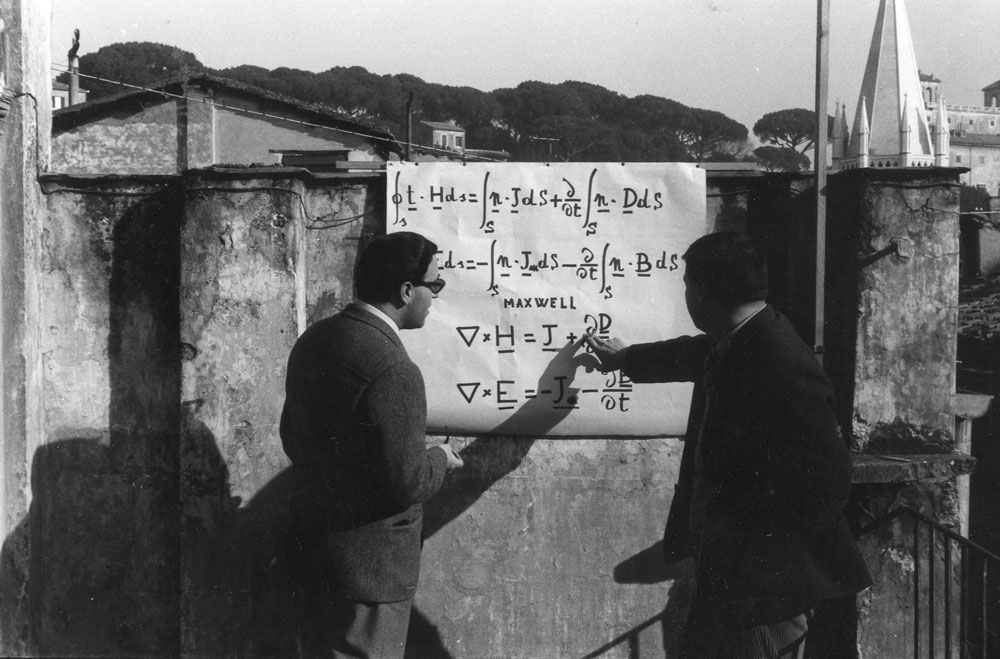
\includegraphics[width=14cm]{figures/EvangelistiNonnis.jpg}
        \caption{Franco Evangelisti e Franco Nonnis sulla terrazza di Vittorio Consoli 
        che osservano le Equazioni di Maxwell, 1959}
        \vspace{0.5cm}
        \end{center}
\end{figure} 

\clearpage

\subsection{Il Feedback}
\label{sec:Il Feedback}
Il feedback, nella sua espressione inglese, 
unisce le due parole \textit{Feed} che significa ‘alimentare’, 
e \textit{Back} ‘all’indietro’. 

\todo[inline,color=green]{puoi evitare di fare traduzioni slegando parole che nella lingua originaria non sono slegabili. limitati a tradurre il concetto. anche perché back separato non significa ciò che hai scritto}

Il primo a introdurre il concetto di feedback nella letteratura scientifica 
è stato lo scienziato inglese James Clerk Maxwell, 
il quale nel 1868 pubblicò uno studio \footcite{maxwellongovernor}
sui sistemi automatici, in cui metteva in evidenza come essi fossero in grado di correggersi
in maniera automatica proprio grazie al concetto del \textit{ritorno di informazione}.
Maxwell anticipò quel concetto che arriverà a maturazione solo molti anni dopo con 
la nascita della cibernetica e con Norbert Wiener, che diede il nome di cibernetica al campo dei suoi studi proprio in onore del lavoro di Maxwell - dal greco \textit{kybernetiké téchne} sta per ‘arte del governare’, a cui si collega il termine inglese \textit{governor} dell'articolo di Maxwell.
In italiano il significato del termine può essere tradotto come ‘retro-alimentazione’
o ‘retro-iniezione’ che ne preservano in qualche modo il significato originale della lingua inglese,
tuttavia in molti preferiscono conservare direttamente la parola inglese feedback. \\
Nella teoria cibernetica, e in genere in tutte le discipline scientifiche che usano approcci di tipo sistemico, quando il Feedback ha un effetto risultante dall’azione di un sistema (meccanismo, circuito, organismo ecc.) che si riflette sul sistema stesso per variarne e correggerne opportunamente il funzionamento, questo si può chiamare Retroazione. \\
Esistono sostanzialmente due tipi di retroazione nel feedback: \textit{positiva} e \textit{negativa}.
Il feedback è generalmente detto negativo quando agisce in modo che il sistema funzioni sempre allo stesso modo, entro margini controllati di tolleranza e convergendo verso un comportamento, viene invece detto positivo quando tende a mantenere il sistema in uno stato di continuo cambiamento.
Tuttavia queste definizioni possono variare da caso a caso, 
e nel corso della tesi ritorneremo su questi temi
riguardo le possibili proprietà del feedback, affrontando queste di volta in volta
nei casi specifici.
Per anticipare da ora alcuni esempi: 
ci basti pensare che nel controllo di un sistema complesso
come può essere quello del feedback elettroacustico,
in un modello dove si possono introdurre delle linearità 
tramite retroazione all'interno del ciclo di
feedback, questo potrebbe ad esempio voler dire costringere la complessità
a dei comportamenti più prevedibili, 
puntando uno stato di convergenza verso l'equilibrio. \\
Un esempio conosciuto è quello dell'intonazione del fenomeno Larsen,
che da un comportamento complesso della sorgente e del ricettore, crescendo
verso la saturazione, per autoscillazione giunge infine ad uno stato stazionario, di stabilità.
Mentre introdurre delle non linearità nel sistema tramite la retroazione,
al contrario, può voler dire portare il sistema verso comportamenti non più prevedibili,
in divergenza dall'equilibrio dello stato stazionario,
e in alcuni casi verso quella che viene chiamata la soglia del caos.
Questi due tipi di comportamento possono essere ottenuti per l'appunto
sia velocizzando che rallentando questi processi
in maniera fortemente dipendente dal caso specifico.
Un secondo esempio può essere invece quello dei filtri digitali audio,
pensati come un valido strumento
di contrasto o avallamento rispetto a questo tipo di comportamenti,
dove se si allineano le fasi si creano dei poli,
mentre se si disallineano si punta generalmente alla complessità del sistema.
Riguardo i filtri digitali basti pensare anche come questi possono essere utilizzati 
negli algoritmi di modellazione fisica
degli strumenti, come ad esempio quello famoso di Karplus-Strong.
Di fatto, concludendo questa introduzione con una visione più generale, 
la storia delle tecnologie elettroacustiche ha
da sempre incorporato il principio del feedback sin dalle sue origini e da prima della
nascita della cibernetica.

\todo[inline,color=green]{hai puntato la data della prima introduzione del feedback a maxwell, 1868… ora non credo tu possa parlare di elettroacustica in quel periodo}

Possiamo pensare a tecnologie
come il triodo, chiamato inizialmente valvola audion di Lee De Forest,
o i circuiti di feedback negativo - negative feedback amplifier - di Harold Black
\footcite{haroldblackamplifier}.

\todo[inline,color=green]{perché citare un componente a caso?}
In sintesi, il principio del feedback continua a essere un pilastro fondamentale nella storia 
e nell'evoluzione delle tecnologie elettroacustiche, 
fino ad essere diventato un aspetto integrato e non più occasionale 
nella prassi dei compositori musicali elettroacustici.